\documentclass[10pt]{article}

\renewcommand{\arraystretch}{1.5}

\usepackage[margin=3cm]{geometry}
\usepackage{gensymb}
\usepackage{csquotes}
\usepackage{hyperref}
\usepackage{graphicx}
\usepackage{subcaption}
\usepackage{amsmath}
\usepackage{amssymb}

\title{Preliminary analysis of data provided by Kaiser Karim}
\author{Alexander Shtyrov\footnote{Email: \texttt{as2875@cam.ac.uk}. Please contact me if you have any questions.}}

\begin{document}
\maketitle

\section{Introduction}
\par The use of multi-electrode arrays (MEAs) to analyse the activity of networks of neurons proliferating \textit{in vitro} has become a common approach in neurophysiology. Most recently, an increased understanding of the transcription factors involved in differentiation of stem cells into neurons has allowed neurons derived from human embryonic stem cells (hESCs) and human induced pluripotent stem cells (hiPSCs) to be cultured on MEAs.

\section{Methods}
\par Kaiser Karim kindly provided a dataset obtained from MEAs containing such cultures for analysis. The protocol used in preparing cells and obtaining recordings is given below.

\begin{displayquote}
For recordings, MEAs incubated at 37 \degree C, 5\% CO\textsubscript{2} were transferred to the MEA recording device (MEA2100-2x60-System, Multichannel Systems). All recordings were performed in atmospheric conditions with stage and custom-built heated lid held at 37 \degree C. Developmental time course recordings took place every second or third day, 10 min after a 37 \degree C, 5\% CO\textsubscript{2} incubation following half-media change. MEAs were allowed to equilibrate for 200 sec on the MEA recording device and recording sessions lasted 10 min with local field potentials from all electrodes sampled at 25 kHz.
\end{displayquote}

\par There were two biological replicates, and three recording attempts \cite{karim_personal_2020}.

\par The data were provided in a format written by MC\_DataTool \cite{multichannel_systems_mc_datatool_2014}. The data were first converted to a data package based on the Frictionless Data Tabular Data Package specification \cite{walsh_tabular_2017}. Each spike was represented by a single timestamp, chosen to be time of the 25\textsuperscript{th} voltage measurement from the start of the spike. Conversion took place via an HDF5 format \cite{eglen_data_2014}.

\par After conversion the data were analysed using a series of Python scripts to compute summary statistics and interspike intervals (ISIs), carry out burst analysis, and extract network spikes. The conversion and analysis scripts will be made available shortly. They make use of the \texttt{elephant} package \cite{elephant_authors_and_contributors_elephant_2020}.

\paragraph{Summary statistics} The summary statistics calculated were: population firing rate, number of spikes recorded, number of active channels, recording time, and firing rate per channel.

\paragraph{ISI histograms} ISIs were calculated for each channel in each recording. Histograms were plotted to show the distribution of ISIs. The bin width of the histograms was calculated by the recommended method in \texttt{matplotlib} \cite{the_scipy_community_numpyhistogram_bin_edges_2020}. This computes the binwidth using two estimators: Freedman-Diaconis (bin width is inversely proportional to the cube root of the sample size) and Sturges (inversely proportional to the logarithm of the sample size). The minimum bin width of the two is then used.

\paragraph{Correlation} The spike time tiling coefficient (STTC) \cite{cutts_detecting_2014} was calculated for each pair of channels in each recording. A synchronicity window of 50 ms was used. The mean coefficient was plotted against age. Channels with an activity of less than 0.5 spikes per minute were excluded from STTC calculations.

\paragraph{Burst analysis} Burst analysis was carried out using an implementation of the MaxInterval method from NeuroExplorer, using the following parameters: a beginning ISI of 0.17 s, an end ISI 0.3 s, a minimum interburst interval (IBI) of 0.2 s, a minimum burst duration of 0.05 s, and a minimum of 3 spikes per burst. The parameters are those recommended in the NeuroExplorer manual \cite{nex_technologies_neuroexplorer_2020}. Raster plots with bursts represented by coloured lines were produced. Box plots showing statistics of bursting behaviour over developmental time were also plotted. The statistics were: frequency of bursts, burst duration, firing rate in bursts, and \% spikes in bursts. Channels with an activity of fewer than 10 spikes per minute were excluded from bursting statistics.

\paragraph{Network spikes} Finally, network spikes were detected using a method similar to the one described by Eytan and Marom \cite{eytan_dynamics_2006}. Spikes were placed in bins, with spikes occurring after the final bin discarded. The number of spikes in each bin was plotted. A network spike occurred when the number of action potentials in a bin exceeded one quarter of the total number of active channels. The 300 ms around the bin were extracted and plotted. Changing the bin width altered the number of detected network spikes, but heuristically it was found that bin widths below 10 ms or above 20 ms abrogated the shape of the extracted spike. Fixing the bin width at 20 ms, the number of network spikes was plotted against age.

\par Raster plots, plots of active channels, and plots of instantaneous firing rate against time were also produced from the raw data for comparison with the analysis of the data converted into the Frictionless format.

\section{Results}

\begin{figure}
	\centering
\begin{subfigure}[b]{0.45\textwidth}
	\centering
	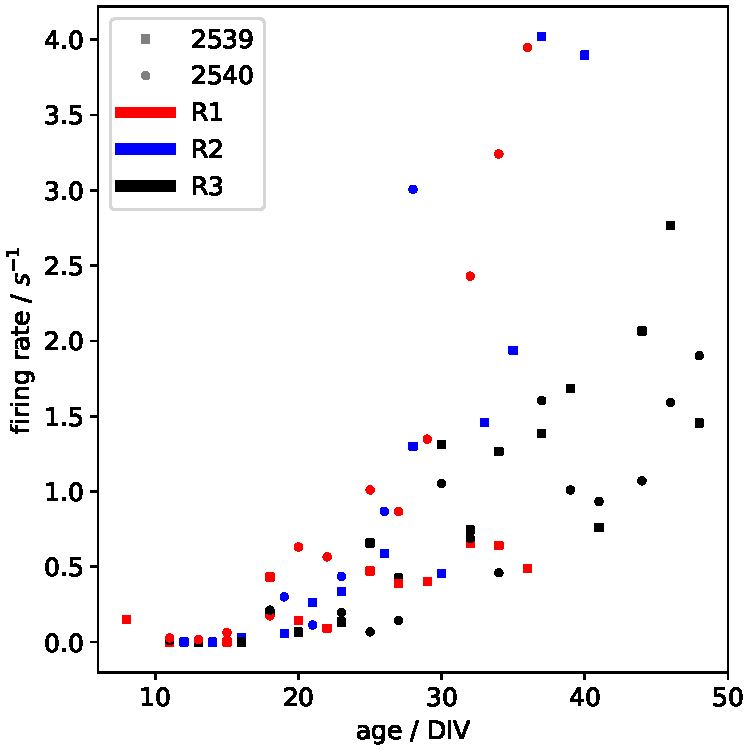
\includegraphics[width=\textwidth]{/home/ashtyrov/Documents/neurofrictionless/plots/development_plots_fr.pdf}
\end{subfigure}
\hfill
\begin{subfigure}[b]{0.45\textwidth}
	\centering
	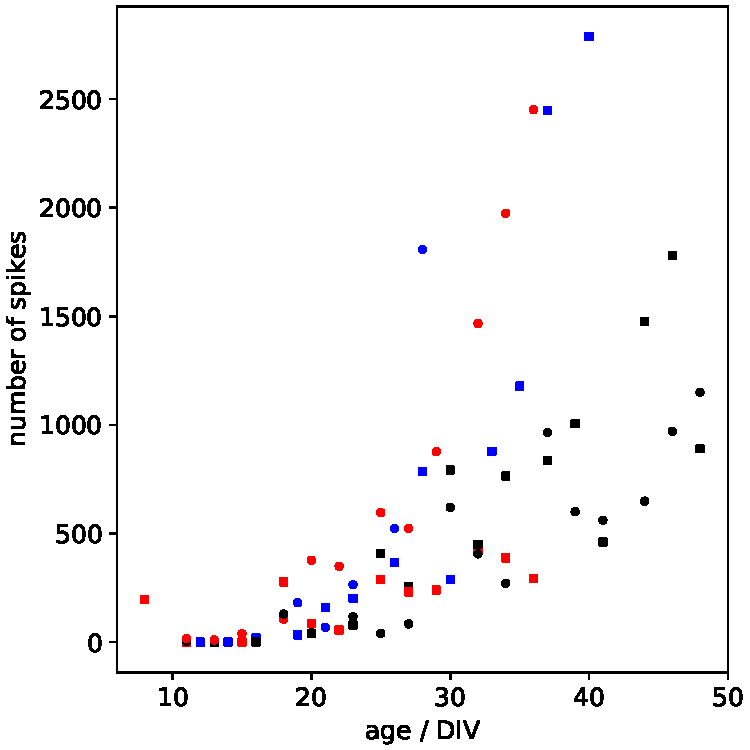
\includegraphics[width=\textwidth]{/home/ashtyrov/Documents/neurofrictionless/plots/development_plots_n.pdf}
\end{subfigure}

\begin{subfigure}[b]{0.45\textwidth}
	\centering
	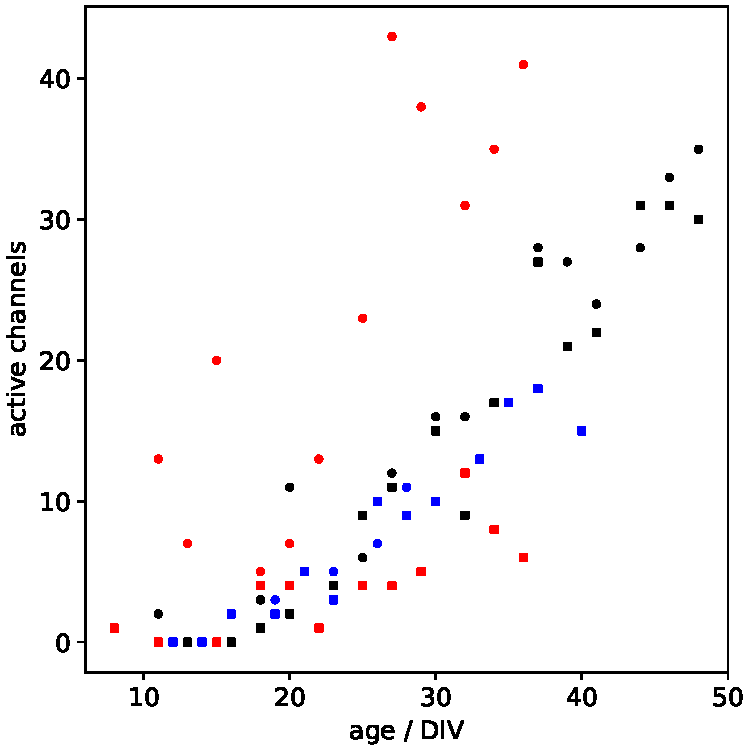
\includegraphics[width=\textwidth]{/home/ashtyrov/Documents/neurofrictionless/plots/development_plots_channels.pdf}
\end{subfigure}
\hfill
\begin{subfigure}[b]{0.45\textwidth}
	\centering
	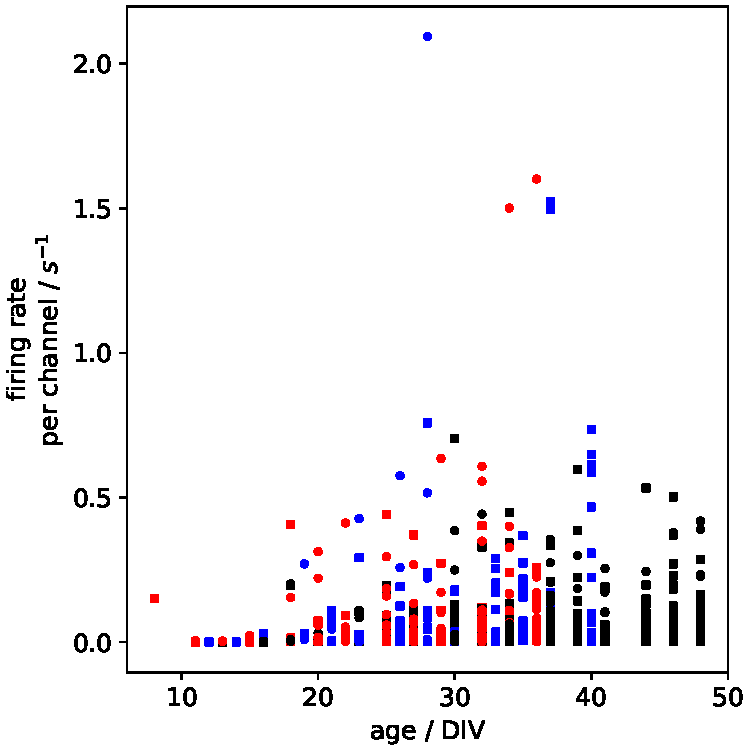
\includegraphics[width=\textwidth]{/home/ashtyrov/Documents/neurofrictionless/plots/development_plots_fr_perchan.pdf}
\end{subfigure}

\begin{subfigure}[b]{0.45\textwidth}
	\centering
	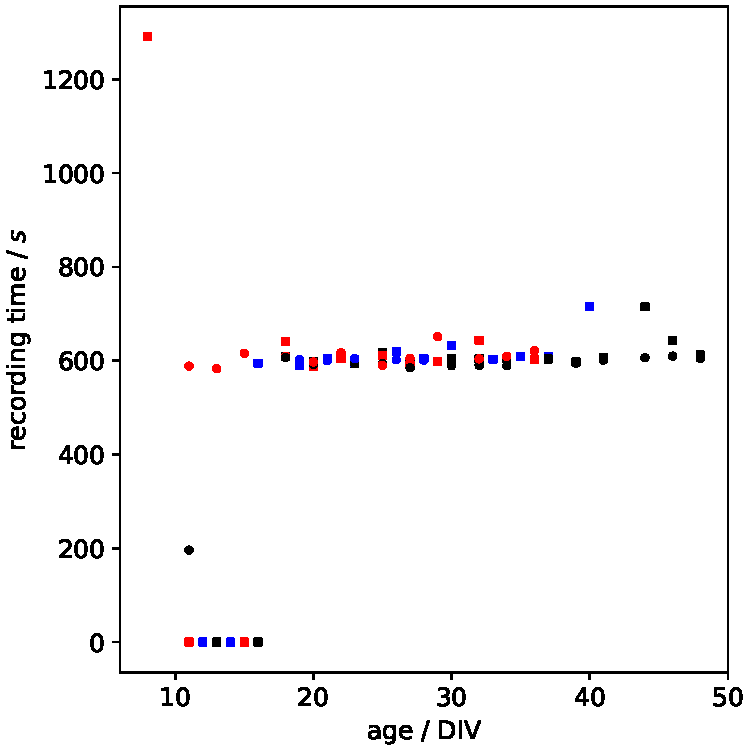
\includegraphics[width=\textwidth]{/home/ashtyrov/Documents/neurofrictionless/plots/development_plots_recording_time.pdf}
\end{subfigure}

	\caption{Plots of network firing rate, number of spikes, number of active channels, recording time, and mean firing rate per channel against age. The main factor in the increase in firing rate is an increase in the number of active channels.}
	\label{fig:development}
\end{figure}

\begin{figure}
	\centering
	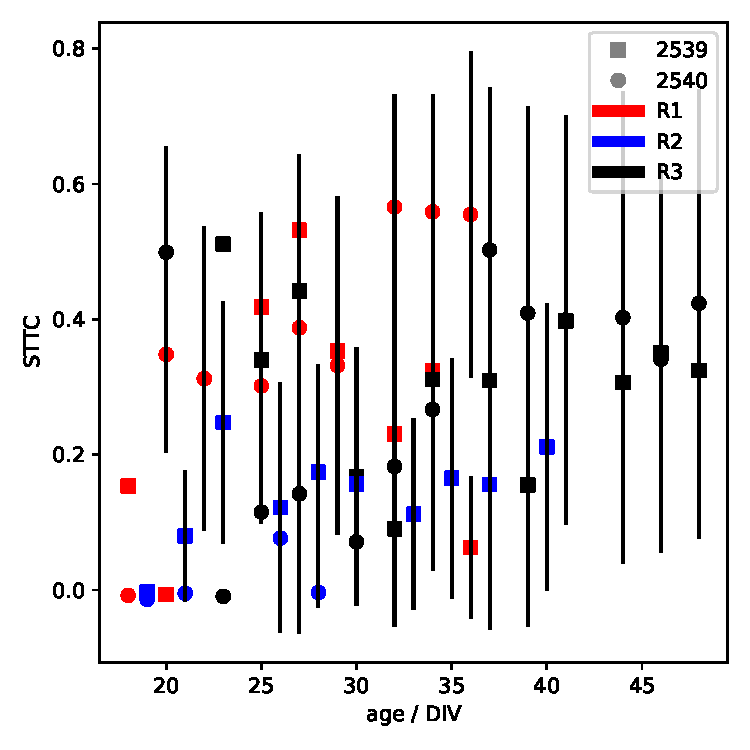
\includegraphics[width=\textwidth]{/home/ashtyrov/Documents/neurofrictionless/plots/correlation_plots.pdf}
	\caption{Plots of mean STTC, calculated pairwise with a synchronicity window of 50 ms, against age. There is no discernible trend in correlation over time.}
	\label{fig:correlation}
\end{figure}

\begin{figure}
	\centering
	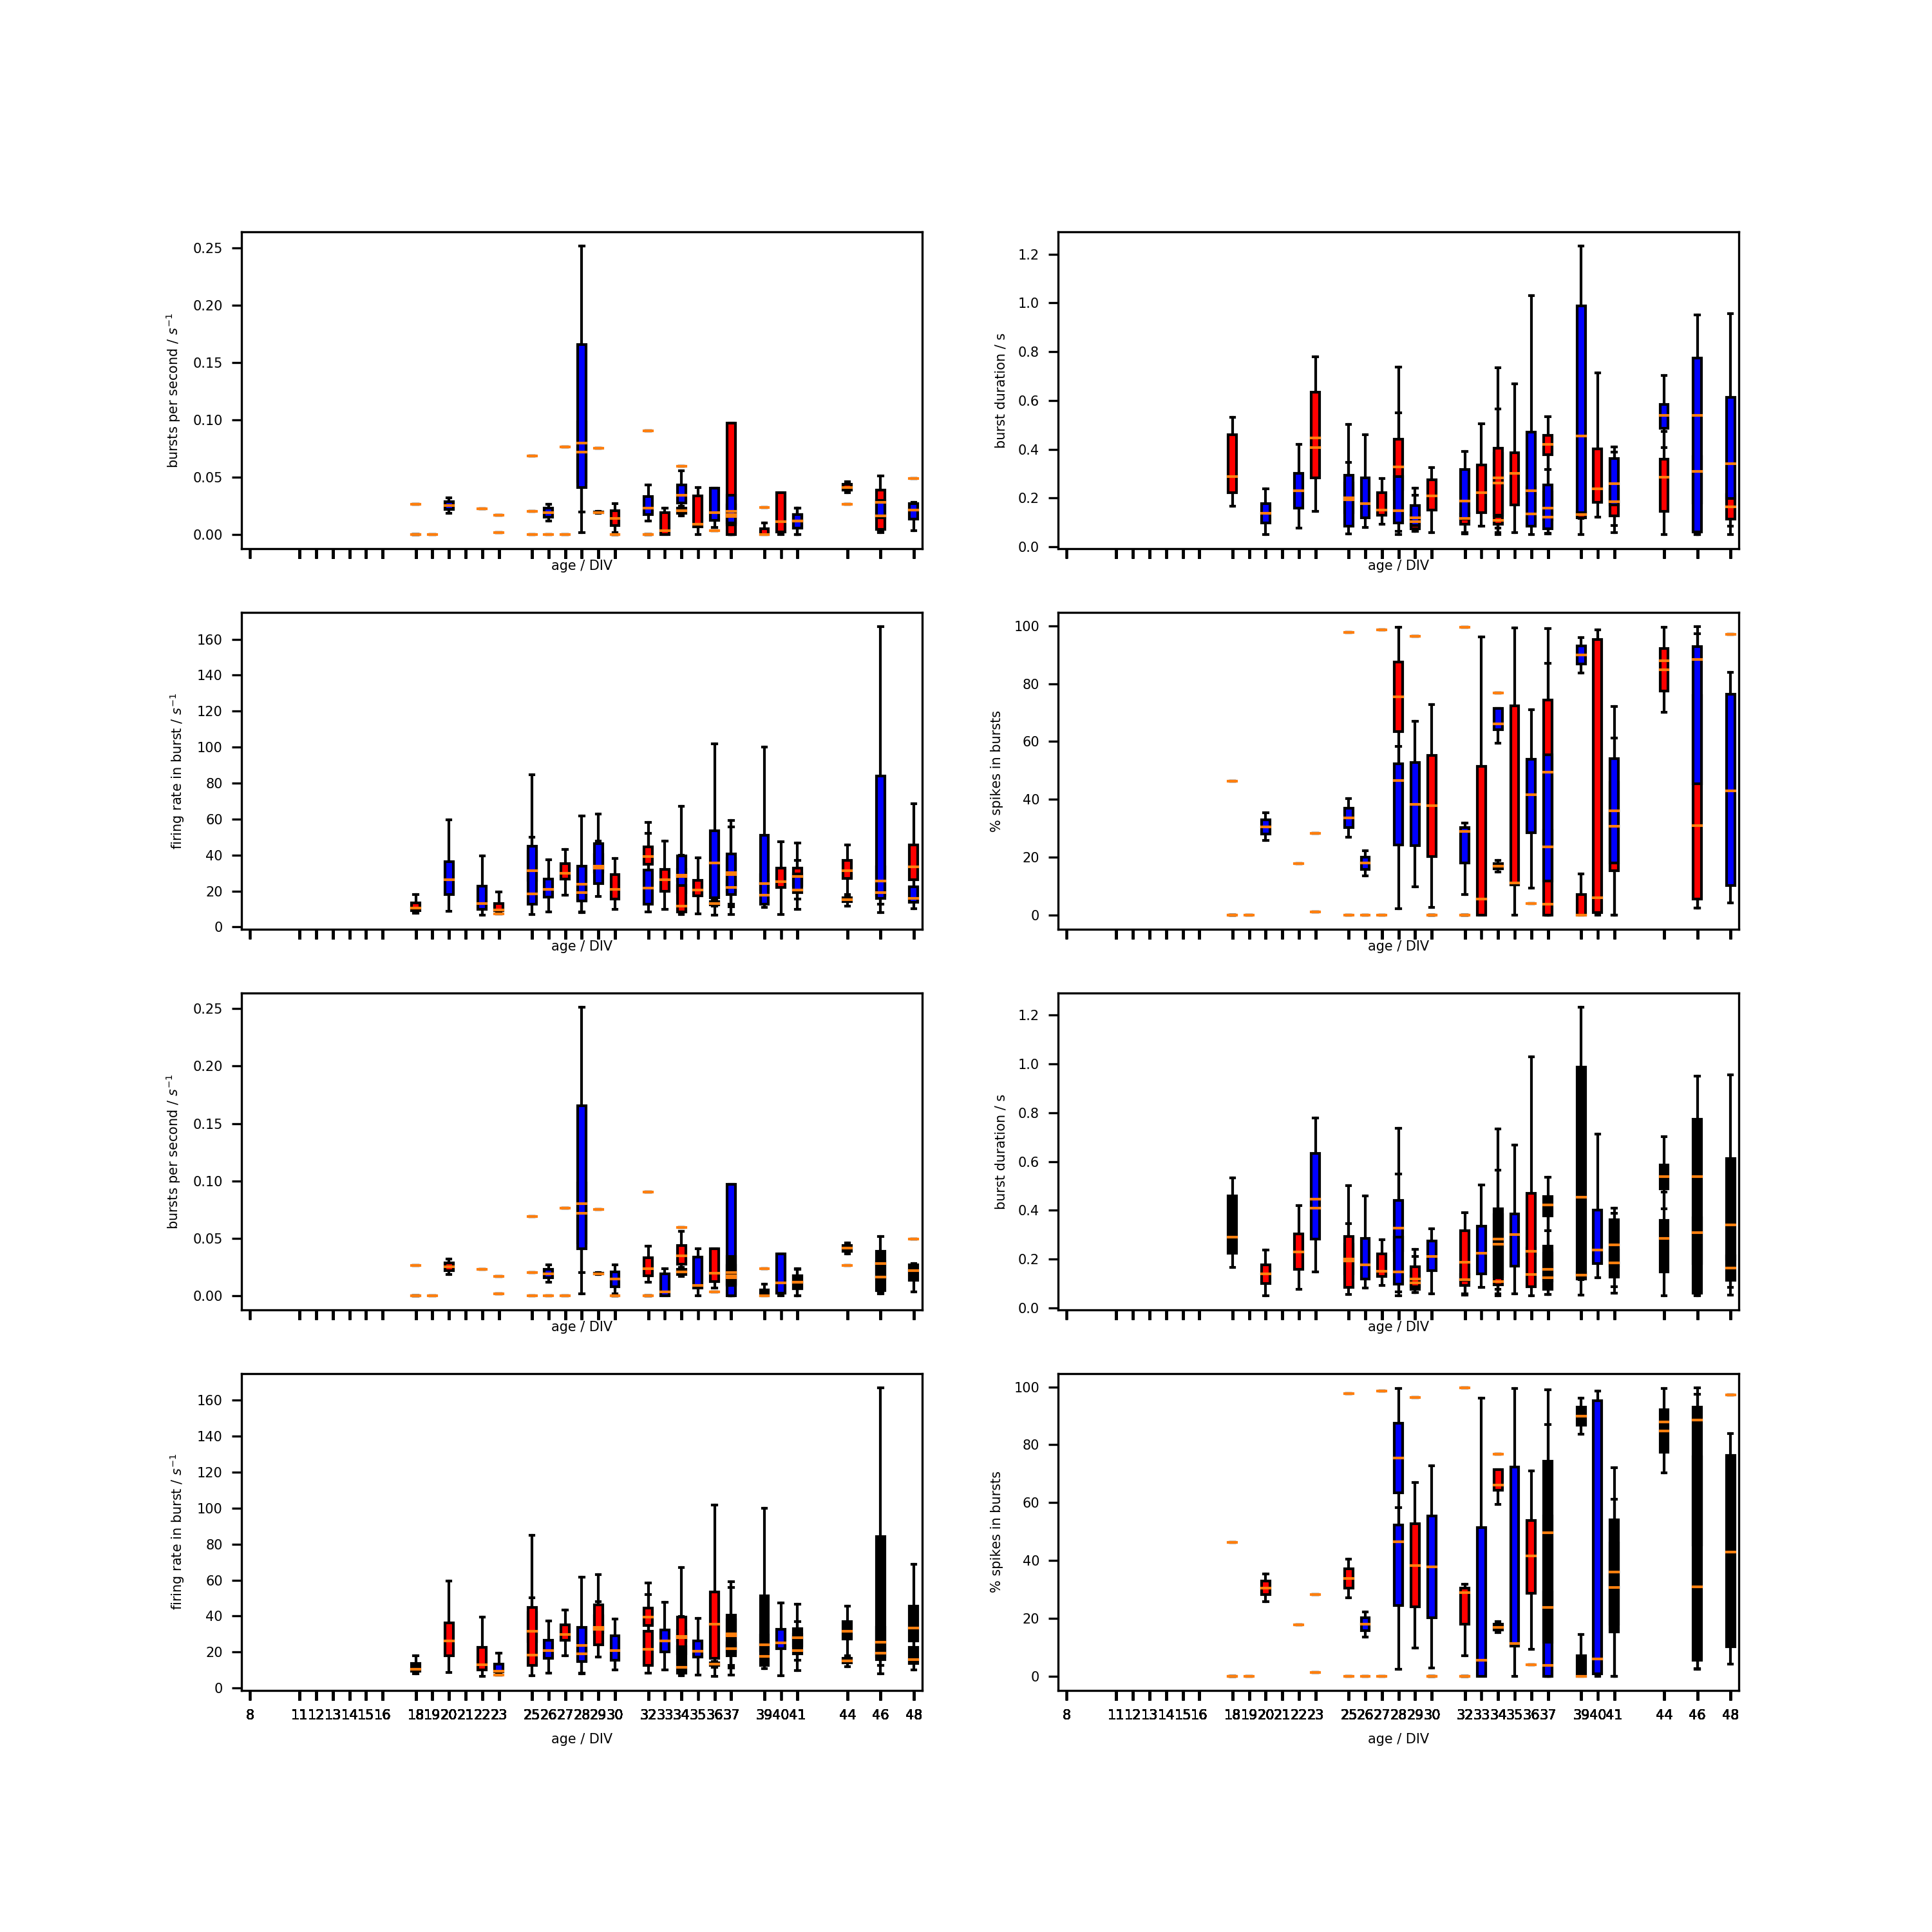
\includegraphics[width=\textwidth]{/home/ashtyrov/Documents/neurofrictionless/plots/burst_boxplots.png}
	\caption{Box plots illustrating bursting behaviour: frequency of bursts, frequency of firing within bursts, burst duration, and proportion of spikes within bursts. Each box is a single recording. Colours are as above.}
	\label{fig:burst}
\end{figure}

\begin{figure}
\centering
\begin{subfigure}[b]{0.7\textwidth}
	\centering
	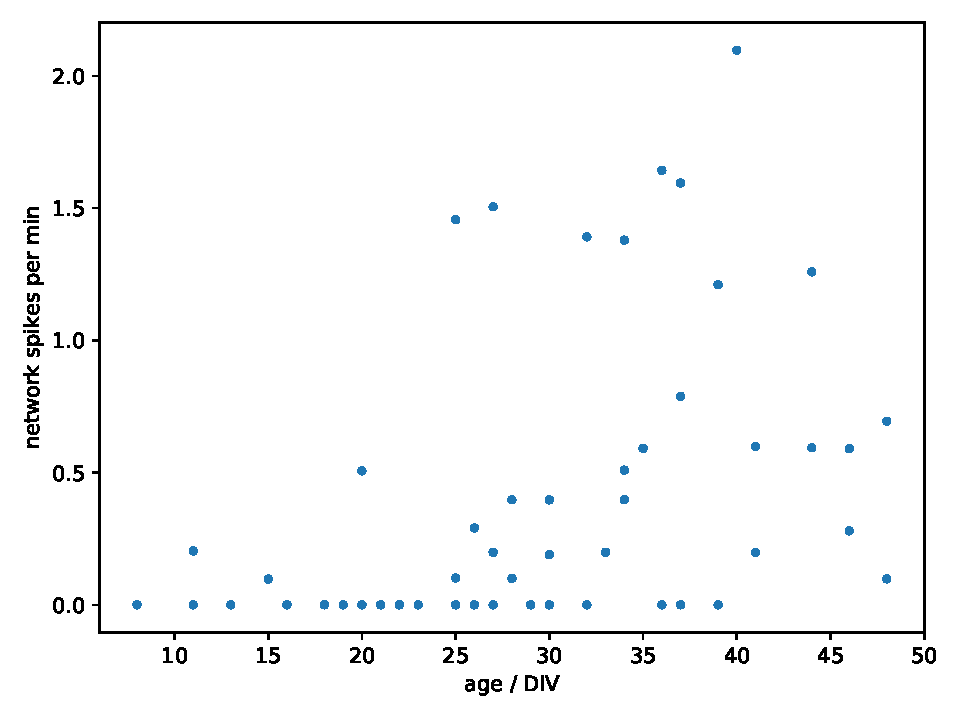
\includegraphics[width=\textwidth]{/home/ashtyrov/Documents/neurofrictionless/plots/network_spikes_age.pdf}
	\caption{The rate of network spike occurrence plotted against age.}
	\label{fig:networkfreq}
\end{subfigure}

\begin{subfigure}[b]{0.7\textwidth}
	\centering
	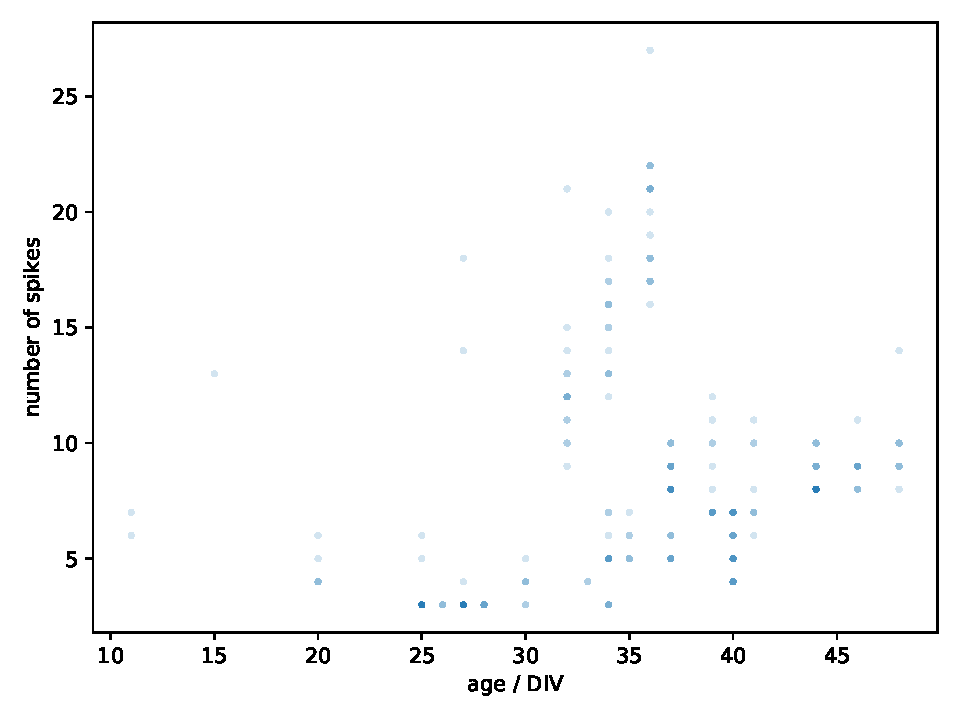
\includegraphics[width=\textwidth]{/home/ashtyrov/Documents/neurofrictionless/plots/network_spikes_amplitude.pdf}
	\caption{The amplitude of network spikes plotted against age.}
	\label{fig:networkamp}
\end{subfigure}
\caption{Characteristics of network spikes.}
\end{figure}

\par The complete set of raster and network activity plots is found in separate files.

\paragraph{Firing rate} Plots of firing rate against developmental time (Figure \ref{fig:development}) show that firing rate increases with time. The number of active channels also increases with time and the firing rate per channel stays approximately constant, suggesting the main factor in firing rate increase is an increase in the number of active channels.

\paragraph{Correlation} There was no clear trend in STTC over time (Figure \ref{fig:correlation}), but firing is correlated throughout development. Varying the length of the synchronicity window scaled the STTCs, but did not affect the overall trend.

\paragraph{ISI} The ISI histograms show frequency density against the natural logarithm of the ISI (Supplementary Figure \ref{fig:histograms}). For all but a few of the most active channels, a bi- or trimodal distribution of ISIs is not observed. This would be the case in samples that have clear bursting behaviour \cite{charlesworth_quantitative_2015}, with the maxima representing modal ISI within bursts and modal IBI (there are two IBIs when bursts of bursts are observed). It may be that the recordings are too short, there are not enough recordings, or there is too much noise.

\paragraph{Burst detection} Unsurprisingly, burst detection showed no clear patterns of bursting, as can be seen in the box plots (Figure \ref{fig:burst}). Examination of the raster plots with bursts highlighted showed that burst detection did not work optimally on these recordings (Supplementary Figure \ref{fig:rasters}). The lack of a distribution of ISIs associated with bursting suggests that changing parameters or detection method would have no effect on the quality of burst detection.

\paragraph{Network spikes} There is an overall upwards trend in the occurrence of network spikes (Figure \ref{fig:networkfreq}) and in the amplitude of spikes, defined as the number of individual spikes in the bin corresponding to the peak of the network spike (Figure \ref{fig:networkamp}), over time. Analysis of network spike shape was not possible because the resolution of the extracted spikes was too low. Qualitatively, many recordings exhibited network spikes (such as the one in Supplementary Figure \ref{fig:networkact}).

\bibliographystyle{plain}
\bibliography{references}

\pagebreak

\section{Supplementary Figures}
\setcounter{figure}{0}
\renewcommand{\thefigure}{S\arabic{figure}}

\begin{figure}[h!]
	\centering
	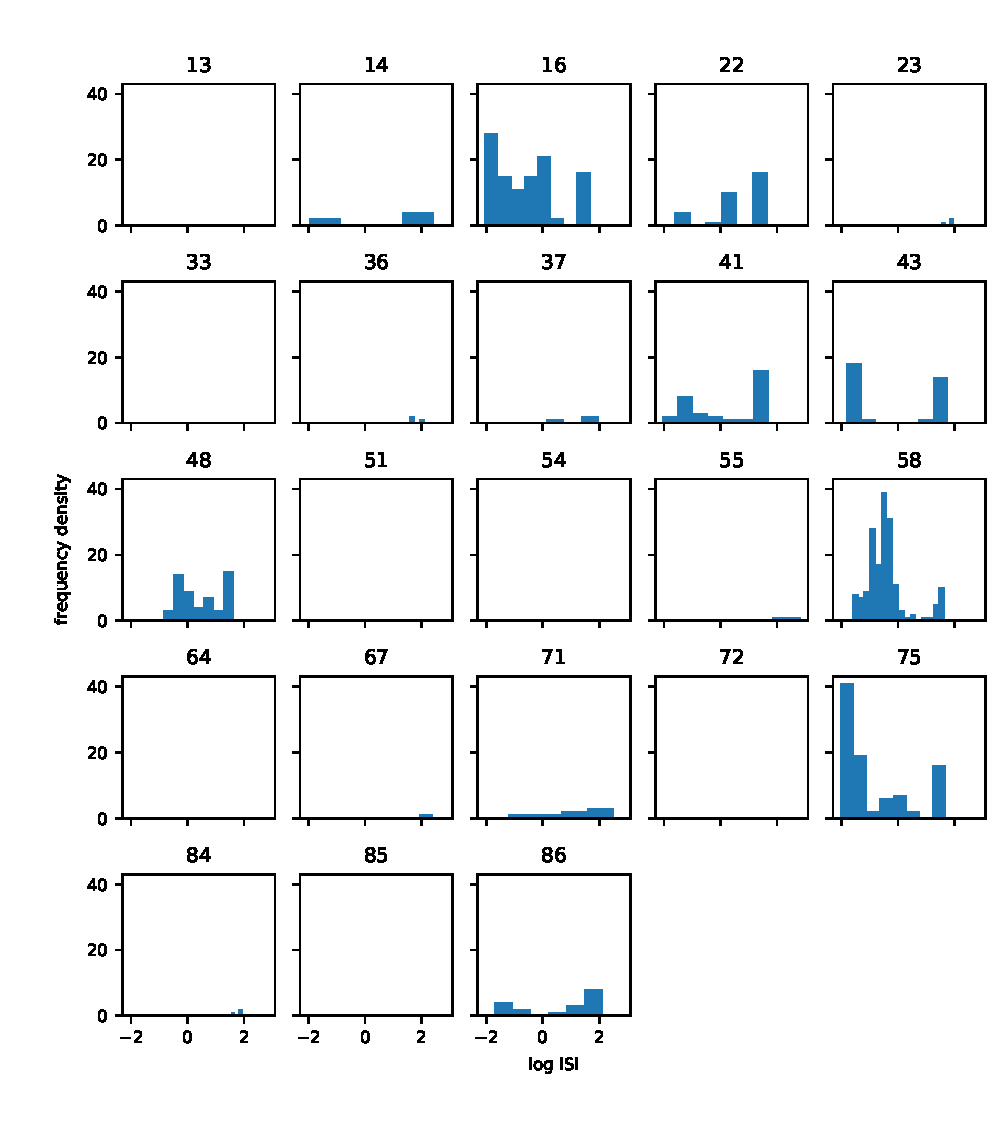
\includegraphics[width=\textwidth]{/home/ashtyrov/Documents/neurofrictionless/plots/supplementary_figures/logisi_plot_example.pdf}
	\caption{A representative set of histograms showing the distribution of ISIs on DIV 36. The \(x\)-axis is \(\log_{10} \text{ISI}\). Although some histograms (such as that of channel 86) show a bimodal distribution, most channels have too few bins for a distribution to be evident.}
	\label{fig:histograms}
\end{figure}

\begin{figure}[h!]
	\centering
	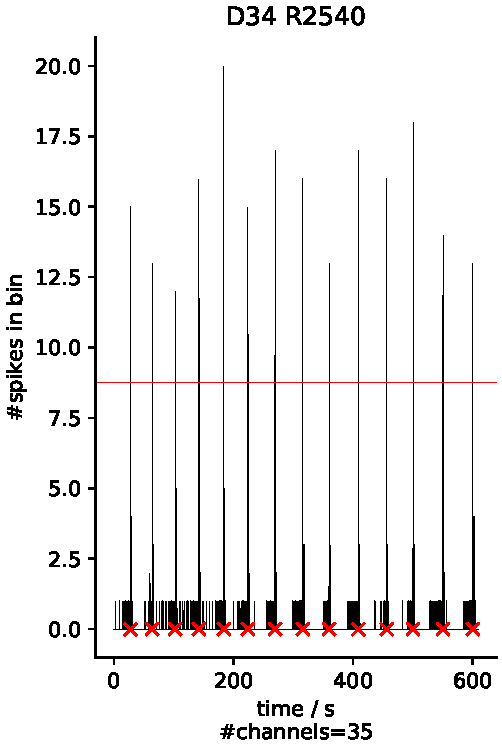
\includegraphics[width=\textwidth]{/home/ashtyrov/Documents/neurofrictionless/plots/supplementary_figures/network_activity_example.pdf}
	\caption{A plot of network activity in a recording against time. The red line is the threshold above which spikes are classed as network spikes. Network spikes are clearly evident. This is DIV 34 of the first recording attempt of sample 2540 with a bin width of 20 ms.}
	\label{fig:networkact}
\end{figure}

\begin{figure}[h!]
\begin{subfigure}{\textwidth}
	\centering
	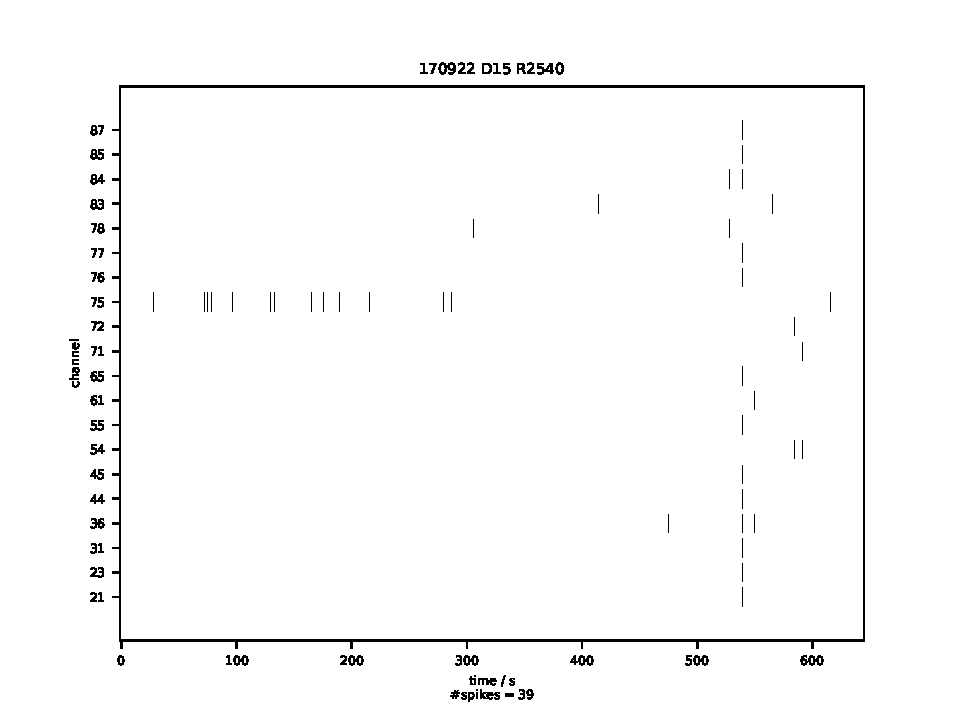
\includegraphics[width=\textwidth]{/home/ashtyrov/Documents/neurofrictionless/plots/supplementary_figures/burst_plot_1.pdf}
	\caption{DIV 15}
\end{subfigure}
\end{figure}

\begin{figure}[h!]
\ContinuedFloat
\begin{subfigure}{\textwidth}
	\centering
	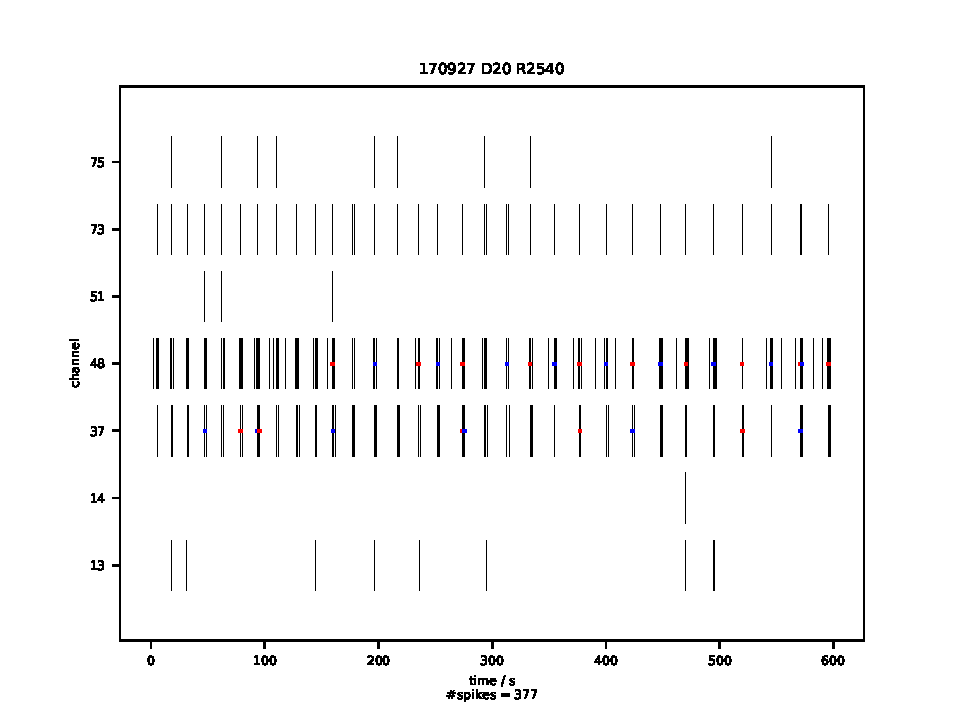
\includegraphics[width=\textwidth]{/home/ashtyrov/Documents/neurofrictionless/plots/supplementary_figures/burst_plot_2.pdf}
	\caption{DIV 20}
\end{subfigure}
\end{figure}

\begin{figure}[h!]
\ContinuedFloat
\begin{subfigure}{\textwidth}
	\centering
	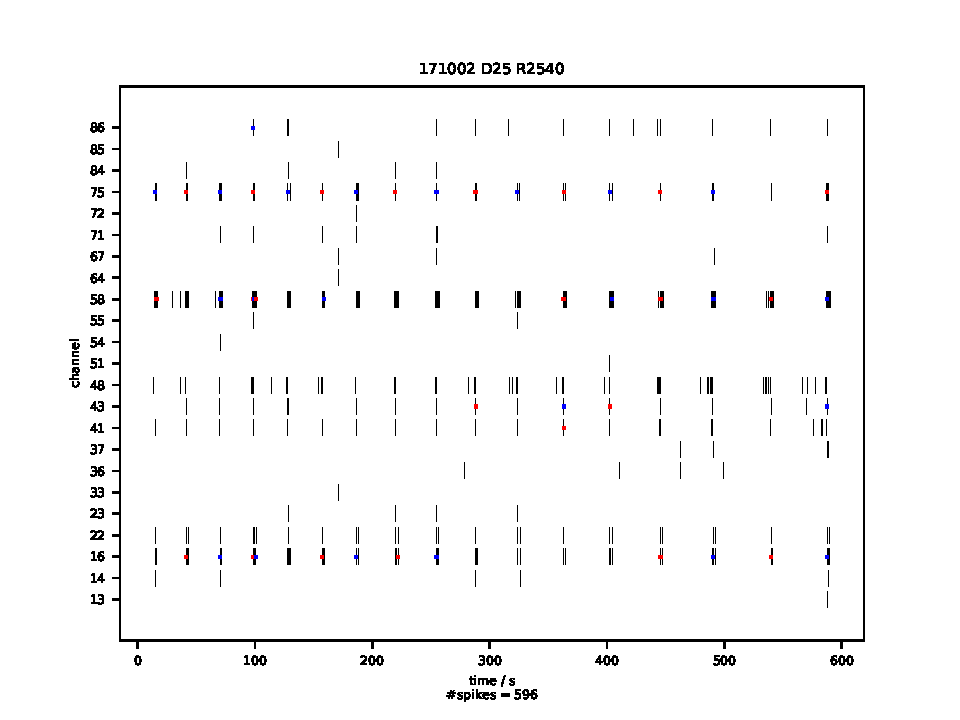
\includegraphics[width=\textwidth]{/home/ashtyrov/Documents/neurofrictionless/plots/supplementary_figures/burst_plot_3.pdf}
	\caption{DIV 25}
\end{subfigure}
\end{figure}

\begin{figure}[h!]
\ContinuedFloat
\begin{subfigure}{\textwidth}
	\centering
	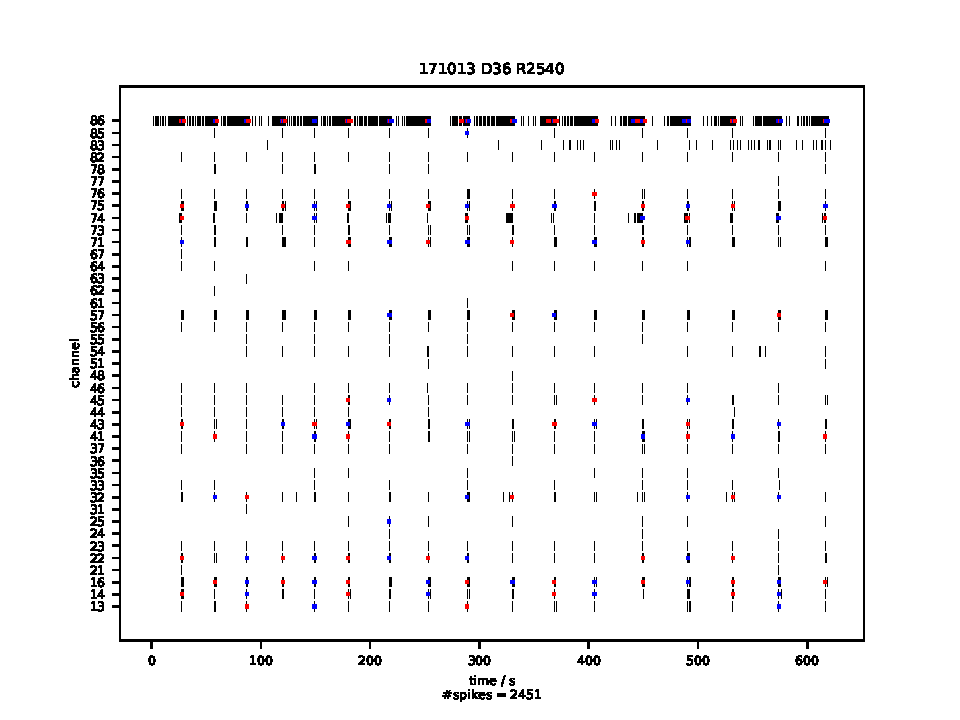
\includegraphics[width=\textwidth]{/home/ashtyrov/Documents/neurofrictionless/plots/supplementary_figures/burst_plot_4.pdf}
	\caption{DIV 36}
\end{subfigure}
\caption{Raster plots showing channel activity at four points in development. Bursts are highlighted with coloured lines. All recordings are from the first recording attempt of replicate 2540.}
\label{fig:rasters}
\end{figure}
\end{document}
